% Capítulo 12: a classe ContaBancaria como molde e dois objetos criados a partir dela.
\documentclass[border=4pt]{standalone}
\usepackage[utf8]{inputenc}
\usepackage[T1]{fontenc}
% Estilo comum dos fluxogramas e diagramas de blocos.
\usepackage{tikz}
\usetikzlibrary{arrows.meta, positioning, calc, shapes.geometric, shapes.misc}
\definecolor{navy}{RGB}{23,45,80}
\definecolor{laranja}{RGB}{250,110,29}
\definecolor{cinzalogo}{RGB}{107,114,126}
\definecolor{azul}{RGB}{205,222,247}
\tikzset{
  base/.style={draw=navy, line width=0.9pt, font=\sffamily\small, align=center, inner sep=4pt},
  terminal/.style={base, rounded rectangle, fill=laranja!45, draw=laranja, minimum width=20mm, minimum height=7mm},
  processo/.style={base, rectangle, fill=laranja!12, minimum width=28mm, minimum height=8mm},
  decisao/.style={base, diamond, aspect=2.2, fill=azul, inner sep=1pt, minimum width=30mm},
  es/.style={base, trapezium, trapezium left angle=72, trapezium right angle=108,
             fill=white, minimum width=26mm, minimum height=8mm, trapezium stretches body},
  fluxo/.style={-{Stealth[length=2.2mm]}, navy, line width=0.9pt},
  rotulo/.style={font=\sffamily\small\bfseries, text=navy},
  legenda/.style={font=\sffamily\scriptsize, text=cinzalogo},
  resposta/.style={font=\sffamily\scriptsize\bfseries, text=navy},
}

\usetikzlibrary{shapes.multipart}
\tikzset{
  classe/.style={rectangle split, rectangle split parts=3, draw=navy, line width=0.9pt,
                 rectangle split part fill={laranja!45, laranja!12, laranja!12},
                 font=\ttfamily\scriptsize, align=left, inner sep=4pt, text width=40mm},
  objeto/.style={rectangle split, rectangle split parts=2, draw=navy, line width=0.9pt,
                 rectangle split part fill={azul, white}, font=\ttfamily\scriptsize,
                 align=left, inner sep=4pt, text width=30mm, rounded corners=2pt},
  instancia/.style={-{Stealth[length=2.2mm]}, navy, line width=0.8pt, dashed},
}
\begin{document}
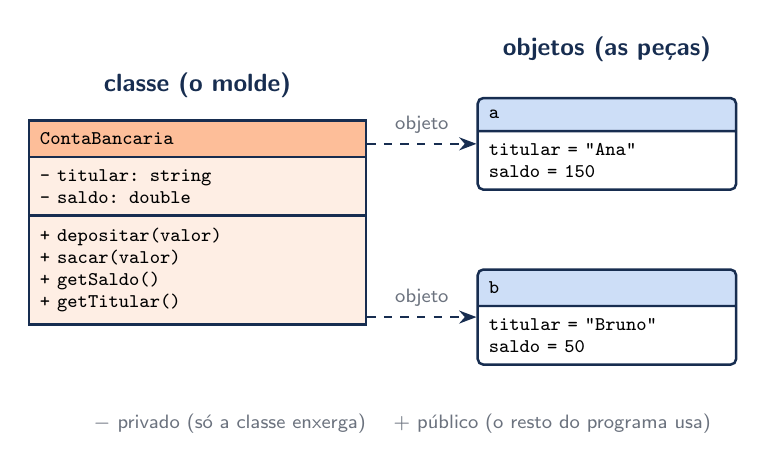
\begin{tikzpicture}
  \node[classe] (c) at (0, 0) {
    \centering\textbf{ContaBancaria}
    \nodepart{two} - titular: string\\- saldo: double
    \nodepart{three} + depositar(valor)\\+ sacar(valor)\\+ getSaldo()\\+ getTitular()};
  \node[objeto] (a) at (5.2, 1.0) {\centering\textbf{a}\nodepart{two}titular = "Ana"\\saldo = 150};
  \node[objeto] (b) at (5.2, -1.2) {\centering\textbf{b}\nodepart{two}titular = "Bruno"\\saldo = 50};
  \draw[instancia] (c.east |- a) -- node[above, legenda] {objeto} (a.west);
  \draw[instancia] (c.east |- b) -- node[above, legenda] {objeto} (b.west);
  \node[rotulo] at (0, 1.75) {classe (o molde)};
  \node[rotulo] at (5.2, 2.2) {objetos (as peças)};
  \node[legenda, align=center] at (2.6, -2.55) {$-$ privado (só a classe enxerga) \quad $+$ público (o resto do programa usa)};
\end{tikzpicture}
\end{document}
